\section{Entropy} \label{sec:shannon_entropy}

% Let's introduce the concept of entropy as a measure of uncertainty of a random variable. A deeper explanation can be found in \cite{han2002mathematics,navarro2016compact,ElementsofInformationTheory}
Let's introduce the concept of entropy as a measure of uncertainty of a random variable. While the worst-case entropy $H_{wc}$, discussed previously, provides a lower bound based solely on the set's cardinality (effectively assuming fixed-length codes or a uniform probability distribution over the elements), Shannon entropy offers a more refined measure. It accounts for the actual probability distribution of the elements, quantifying the \emph{average} uncertainty or information content associated with the random variable. A deeper explanation can be found in \cite{han2002mathematics,navarro2016compact,ElementsofInformationTheory}

\begin{definition}[Entropy of a Random Variable]\label{def:entropy}
    Let $X$ \marginpar{This is also known as Shannon entropy, named after Claude Shannon, who introduced it in his seminal work \cite{Shannon1948}}be a random variable taking values in a finite alphabet $\mathcal{X}$ with the probabilistic distribution $P_X(x)= \text{Pr}\{X=x\}~(x\in\mathcal{X})$. Then, the entropy of $X$ is defined as
    \begin{equation}
        H(X) = H(P_X) \myeq E_{P_x} \{-\log P_X(x)\} = -\sum_{x\in\mathcal{X}} P_X(x)\log P_X(x)
    \end{equation}
\end{definition}
\noindent Where $E_P$ denotes the expectation with respect to the probability distribution $P$. The $\log$ is taken to the base 2 and the entropy is expressed in bits. It is then clear that the entropy of a discrete random variable will always be nonnegative\footnote{The entropy is null if and only if $X = c$, where $c$ is a costant with probability one}. \\



\begin{example}[Toss of a fair coin]
    Let $X$ be a random variable representing the outcome of a toss of a fair coin. The probability distribution of $X$ is $P_X(0) = P_X(1) = \frac{1}{2}$. The entropy of $X$ is
    \begin{equation}
        H(X) = -\frac{1}{2}\log\frac{1}{2} - \frac{1}{2}\log\frac{1}{2} = 1
    \end{equation}
    This means that the toss of a fair coin has an entropy of 1 bit.
\end{example}

\begin{remark}
    Due to historical reasons, we are abusing the notation and using $H(X)$ to denote the entropy of the random variable $X$. It's important to note that this is not a function of the random variable: it's a functional of the distribution of $X$. It does not depend on the actual values taken by the random variable, but only on the probabilities of these values.
\end{remark}

\noindent The concept of entropy, introduced in definition \ref{def:entropy}, helps us quantify the randomness or uncertainty associated with a random variable. It essentially reflects the average amount of information needed to identify a specific value drawn from that variable. Intuitively, we can think of entropy as the average number of digits required to express a sampled value.

% \noindent However, for continuous random variables (variables with an infinite number of possible values), expressing a single value with perfect accuracy requires an infinite number of digits. This is because any finite number of digits will only represent a range of possible values, not a single precise value. As a result, when we apply the definition of entropy to a continuous variable by dividing its range into increasingly smaller intervals and taking the limit, the entropy diverges to infinity.


\subsection{Properties}
In the previous section \ref{sec:shannon_entropy}, we have introduced the entropy of a single random variable $X$. What if we have two random variables $X$ and $Y$? How can we measure the uncertainty of the pair $(X,Y)$? This is where the concept of joint entropy comes into play. The idea is to consider $(X,Y)$ as a single vector-valued random variable and compute its entropy. This is the joint entropy of $X$ and $Y$. To quantify the total uncertainty associated with a pair of variables considered together, we define the joint entropy:

\begin{definition}[Joint Entropy]\label{def:joint_entropy}
    Let $(X,Y)$ be a pair of discrete random variables $(X,Y)$ with a joint distribution $P_{XY}(x,y) = \text{Pr}\{X=x,Y=y\}$. The joint entropy of $(X,Y)$ is defined as
    \begin{equation}\label{eq:joint_entropy}
        H(X,Y) = H(P_{XY}) = -\sum_{x\in\mathcal{X}}\sum_{y\in\mathcal{Y}} P_{XY}(x,y)\log P_{XY}(x,y)
    \end{equation}
\end{definition}
\noindent Which we can be extended to the joint entropy of $n$ random variables $(X_1,X_2,\ldots,X_n)$ as $H(X_1,\ldots, X_n)$. \vspace*{0.4cm}

\noindent We also define the conditional entropy of a random variable given another as the expected value of the entropies of the conditional distributions, averaged over the conditioning random variable.
% Given two random variables $X$ and $Y$, we can define $W(y|x)$, with $x \in \mathcal{X}$ and $y \in \mathcal{Y}$, as the conditional probability of $Y$ given $X$. The set $W$ of those conditional probabilities is called \emph{channel} with \emph{input alphabet} $\mathcal{X}$ and \emph{output alphabet} $\mathcal{Y}$.
Often, it's helpful to conceptualize the relationship between $Y$ and $X$ in terms of information transmission. Given $X$, we can determine the probability of observing $Y$ through the conditional probability $W(y|x) = \text{Pr}\{Y=y|X=x\}$ for all $x \in \mathcal{X}$ and $y \in \mathcal{Y}$. The collection $W$ of these conditional probabilities effectively describes how information about X influences the outcome of Y, and is often referred to as a \emph{channel} with \emph{input alphabet} $\mathcal{X}$ and \emph{output alphabet} $\mathcal{Y}$.

\begin{definition}[Conditional Entropy]\label{def:conditional_entropy}
    Let $(X,Y)$ be a pair of discrete random variables with a joint distribution $P_{XY}(x,y) = \text{Pr}\{X=x,Y=y\}$. The conditional entropy of $Y$ given $X$ is defined as
    \begin{align}
        H(Y|X) & = H(W | P_X) \myeq \sum_x P_X(x)H(Y|x)                                                       \\
               & = \sum_{x \in \mathcal{X}} P_X(x) \Big\{ -\sum_{y \in \mathcal{Y}} W(y|x) \log W(y|x) \Big\} \\
               & = -\sum_{x\in\mathcal{X}}\sum_{y\in\mathcal{Y}} P_{XY}(x,y)\log W(y|x)                       \\
               & = E_{P_{XY}} \{ -\log W(Y|X) \}
    \end{align}
\end{definition}

\noindent Since entropy is always nonnegative, conditional entropy is likewise nonnegative; it has value zero if and only if $Y$ can be entirely determined from $X$ with certainty, meaning there exists a function $f(X)$ such that $Y = f(X)$ with probability one. \vspace*{0.4cm}

\noindent The connection between joint entropy and conditional is more evident when considering that the entropy of two random variables equals the entropy of one of them plus the conditional entropy of the other. This connection is formally proven in the following theorem.

\begin{theorem}[Chain Rule]\label{thm:chain_rule}
    Let $(X,Y)$\marginpar{This is also known as additivity of entropy.} be a pair of discrete random variables with a joint distribution $P_{XY}(x,y)$. Then, the joint entropy of $(X,Y)$ can be expressed as
    \begin{equation}
        H(X,Y) = H(X) + H(Y|X)
    \end{equation}
\end{theorem}
\begin{proof}
    From the definition of conditional entropy (\ref{def:conditional_entropy}), we have
    \begin{align*}
        H(X,Y) & = -\sum_{x,y} P_{XY}(x,y) \log W(y|x)                                        \\
               & = -\sum_{x,y} P_{XY}(x,y) \log \frac{P_{XY}(x,y)}{P_X(x)}                    \\
               & = -\sum_{x,y} P_{XY}(x,y) \log P_{XY}(x,y) + \sum_{x,y} P_{X}(x) \log P_X(x) \\
               & = H(XY) + H(X)
    \end{align*}
    Where we used the relation
    \begin{equation}
        W(y|x) = \frac{P_{XY}(x,y)}{P_X(x)}
    \end{equation}
    When $P_X(x) \neq 0$.
\end{proof}

\begin{corollary}
    \begin{equation}
        H(X, Y|Z) = H(X|Z) + H(Y|X,Z)
    \end{equation}
\end{corollary}
\begin{proof}
    The proof is analogous to the proof of the chain rule.
\end{proof}

\begin{corollary}
    \begin{align}
        H(X_1, X_2, \ldots, X_n) & = H(X_1) + H(X_2|X_1) + H(X_3|X_1, X_2) \nonumber \\
                                 & + \ldots + H(X_n|X_1, X_2, \ldots, X_{n-1})
    \end{align}
\end{corollary}
\begin{proof}
    We can apply the two-variable chain rule in repetition obtain the result.
\end{proof}

\subsection{Mutual Information}
Given two random variables $X$ and $Y$, the mutual information between them quantifies the reduction in uncertainty about one variable due to the knowledge of the other. It is defined as the difference between the entropy and the conditional entropy. Figure \ref{fig:mutual_information} illustrates the concept of mutual information between two random variables. We've seen how to measure the uncertainty of individual variables and pairs. But how much does knowing one variable tell us about the other? In other words, how much uncertainty about $X$ is removed by knowing $Y$? This is quantified by the mutual information:

\begin{definition}[Mutual Information]\label{def:mutual_information}
    Let $(X,Y)$ be a pair of discrete random variables with a joint distribution $P_{XY}(x,y)$. The mutual information between $X$ and $Y$ is defined as
    \begin{equation}
        I(X;Y) = H(X) - H(X|Y)
    \end{equation}
\end{definition}
\noindent Using the chain rule (\ref{thm:chain_rule}), we can rewrite it as
\begin{align}
    I(X;Y) & = H(X) - H(X|Y) \nonumber                                           \\
           & = H(X) + H(Y) - H(X,Y)                                              \\
           & = -\sum_x P_X(x)\log P_X(x) - \sum_y P_Y(y)\log P_Y(y) \nonumber    \\
           & \quad + \sum_{x,y} P_{XY}(x,y)\log P_{XY}(x,y)                      \\
           & = \sum_{x,y} P_{XY}(x,y)\log \frac{P_{XY}(x,y)}{P_X(x)P_Y(y)}       \\
           & = E_{P_{XY}} \left\{ \log \frac{P_{XY}(x,y)}{P_X(x)P_Y(y)} \right\}
\end{align}
It follows immediately that the mutual information is symmetric, $I(X;Y) = I(Y;X)$.

\begin{figure}[h!]
    \centering
    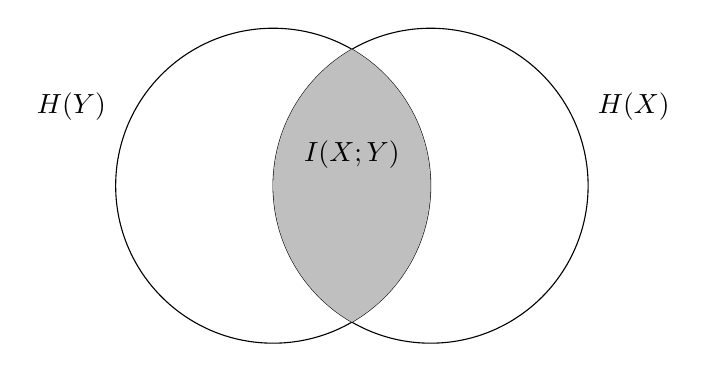
\begin{tikzpicture}
        % Define the circles
        \def\radius{2cm}
        \def\dist{2cm}
        \coordinate (center1) at (0,0);
        \coordinate (center2) at (\dist,0);

        % Draw circles
        \draw (center1) circle [radius=\radius];
        \draw (center2) circle [radius=\radius];

        % Color intersection
        \begin{scope}
            \clip (center1) circle (\radius);
            \fill[lightgray] (center2) circle (\radius);
        \end{scope}

        % Label intersection
        \coordinate (intersection) at (\dist/2,0);
        \node at (intersection) [below, above=0.1cm] {$I(X;Y)$};

        % Move labels outside
        \node at (center1) [above=1cm, left=2cm] {$H(Y)$};
        \node at (center2) [above=1cm, right=2cm] {$H(X)$};
    \end{tikzpicture}
    \caption{Mutual information between two random variables $X$ and $Y$.\label{fig:mutual_information}}
\end{figure}

\subsection{Fano's inequality}

Information theory serves as a cornerstone for understanding fundamental limits in data compression. It not only allows us to prove the existence of encoders (\autoref{sec:source_and_codes}) achieving demonstrably good performance, but also establishes a theoretical barrier against surpassing this performance. The following theorem, known as Fano's inequality, provides a lower bound on the probability of error in guessing a random variable $X$ to it's conditional entropy $H(X|Y)$, where $Y$ is another random variable\footnote{We have seen in \ref{def:conditional_entropy} that the conditional entropy of $X$ given $Y$ is zero if and only if $X$ is a deterministic function of $Y$. Hence, we can estimate $X$ from $Y$ with zero error if and only if $H(X|Y) = 0$.}.

\begin{theorem}[Fano's Inequality]\label{thm:fano_inequality}
    Let $X$ and $Y$ be two discrete random variables with $X$ taking values in some discrete alphabet $\mathcal{X}$, we have
    \begin{equation}
        H(X|Y) \leq \text{Pr}\{X \neq Y\} \log (|\mathcal{X}|-1) + h(\text{Pr}\{X \neq Y\})
    \end{equation}
    where $h(p) = -p\log p - (1-p)\log(1-p)$ is the binary entropy function.
\end{theorem}
\begin{proof}
    Let $Z$ be a random variable defined as follows:
    \begin{equation}\label{eq:random_variable_Z}
        Z = \begin{cases}
            1 & \text{if } X \neq Y \\
            0 & \text{if } X = Y
        \end{cases}
    \end{equation}
    We can then write
    \begin{align} \label{eq:entropy_decomposition}
        H(X|Y) & = H(X|Y) + H(Z|XY) = H(XZ|Y) \nonumber \\
               & = H(X|YZ) + H(Z|Y) \nonumber           \\
               & \leq H(X|YZ) + H(Z)
    \end{align}
    The last inequality follows from the fact that conditioning reduces entropy. We can then write
    \begin{equation} \label{eq:entropy_decomposition2}
        H(Z) = h(\text{Pr}\{X \neq Y\})
    \end{equation}
    Since $\forall y \in \mathcal{Y}$, we can write
    \begin{equation}
        H(X | Y =y, Z =0) =0
    \end{equation}
    and
    \begin{equation}
        H(X| Y = y, Z = 1) \leq \log(|\mathcal{X}|-1)
    \end{equation}
    Combining these results, we have
    \begin{equation} \label{eq:entropy_decomposition3}
        H(X | YZ) \leq \text{Pr}\{X \neq Y\} \log (|\mathcal{X}|-1)
    \end{equation}
    From equations \ref{eq:entropy_decomposition}, \ref{eq:entropy_decomposition2} and \ref{eq:entropy_decomposition3}, we have Fano's inequality.
\end{proof}
% \todo[inline]{Add some conclusions to this section.}
\noindent Fano's inequality thus provides a tangible link between the conditional entropy $H(X|Y)$, which quantifies the remaining uncertainty about $X$ when $Y$ is known, and the minimum probability of error achievable in any attempt to estimate $X$ from $Y$. This inequality, along with the foundational concepts of entropy, joint entropy, conditional entropy, and mutual information introduced throughout this section, establishes a robust theoretical framework. These tools are not merely abstract measures; they allow us to quantify information, understand dependencies between data sources, and ultimately, to delineate the fundamental limits governing how efficiently data can be represented and compressed. Understanding these limits is essential as we delve deeper into specific encoding techniques.
\clearpage
